\section{Continuity}\label{sec:Continuity}

The graph shown in Figure \ref{fig:continuousfunc}(a) represents a
\dfont{continuous} function.  Geometrically, this is because there are no
jumps in the graphs.  That is, if you pick a point on the graph and
approach it from the left and right, the values of the function approach
the value of the function at that point.  For example, we can see that this
is not true for function values near $x=1$ on the graph in Figure \ref{fig:continuousfunc}(b) which is
not continuous at that location.

\figure[!ht]
$$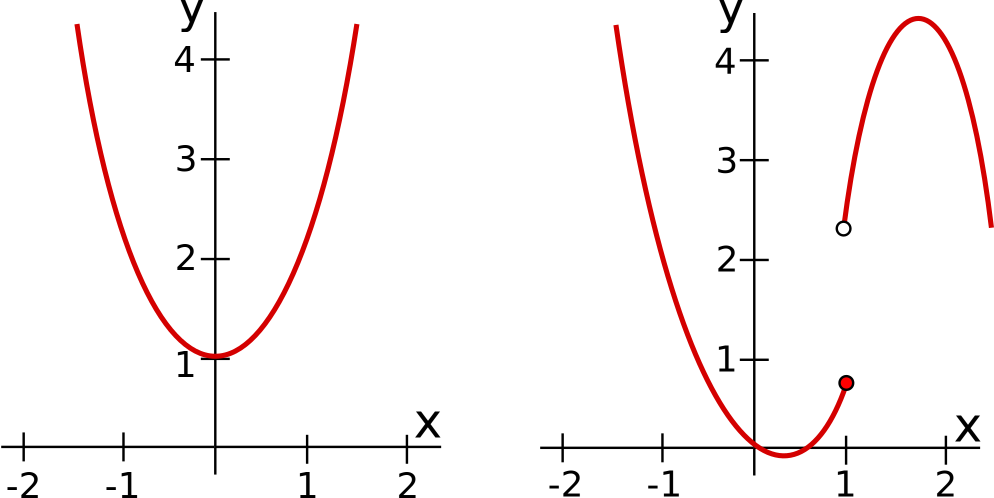
\includegraphics[width=4.0in]{images/continuous}$$
\caption{(a) A continuous function. (b) A function with a discontinuity at $x=1$. \label{fig:continuousfunc}}
\endfigure

\begin{definition}{Continuous at a Point}{ContinuousPoint}
A function $f$ is \deffont{continuous
at a point $a$} if $$\ds \lim_{x\to a} f(x) = f(a).$$
\end{definition}

Some readers may prefer to think of continuity at a point as a three part definition.
That is, a function $f(x)$ is continuous at $x=a$ if the following three conditions hold:
\begin{enumerate}[(i)]
	\item $f(a)$ is defined (that is, $a$ belongs to the domain of $f$),
	\item $\ds{\lim_{x\to a}f(x)}$ exists (that is, left-hand limit $=$ right-hand limit),
	\item $\ds{\lim_{x\to a}f(x)=f(a)}$ (that is, the numbers from (i) and (ii) are equal).
\end{enumerate}

The figures below show graphical examples of functions where either (i), (ii) or (iii) can fail to hold.

$$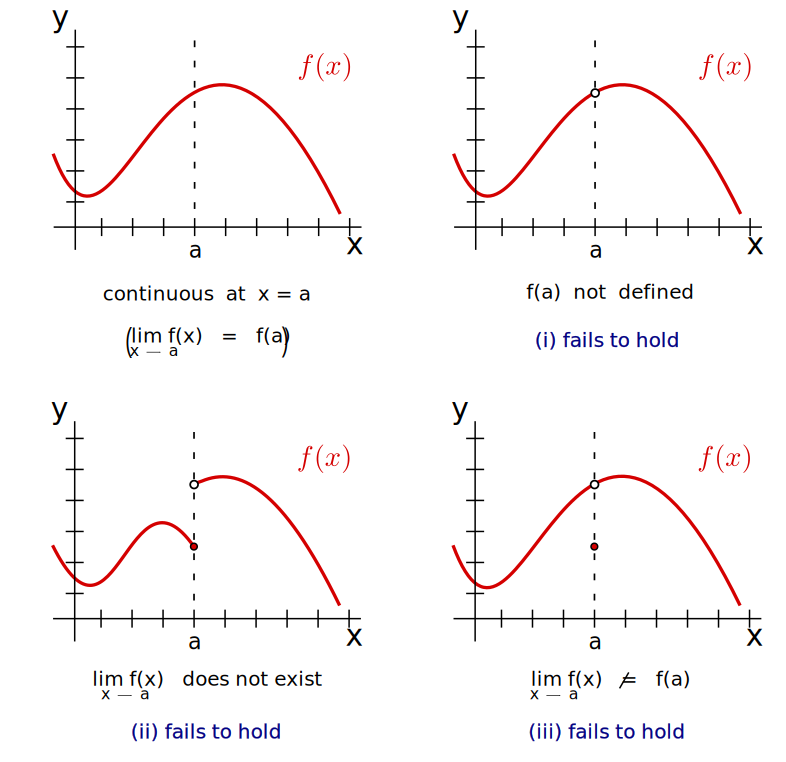
\includegraphics[width=6.5in]{images2/continuity-3-part}$$

On the other hand, if $f$ is defined on an open interval containing $a$, except perhaps at $a$, we can say that $f$ is \dfont{discontinuous} at $a$ if $f$ is not continuous at $a$.

Graphically, you can think of continuity as being able to draw your function without having to lift your pencil off the paper. If your pencil has to jump off the page to continue drawing the function, then the function is not continuous at that point.
This is illustrated in Figure \ref{fig:continuousfunc}(b) where if we tried to draw the function (from left to right) we need to lift our pencil off the page once we reach the point $x=1$ in order to be able to continue drawing the function.

\begin{definition}{Continuity on an Open Interval}{ContinuousOpenIntervalDefinition}
A function $f$ is \deffont{continuous on an open interval $(a,b)$} if it is continuous at every point in the interval.

\medskip
Furthermore, a function is \deffont{everywhere continuous} if it is continuous on the entire real number line $(-\infty,\infty)$..
\end{definition}

Recall the function graphed in a previous section as shown in Figure \ref{fig:discontgraph}.

\figure[!ht]
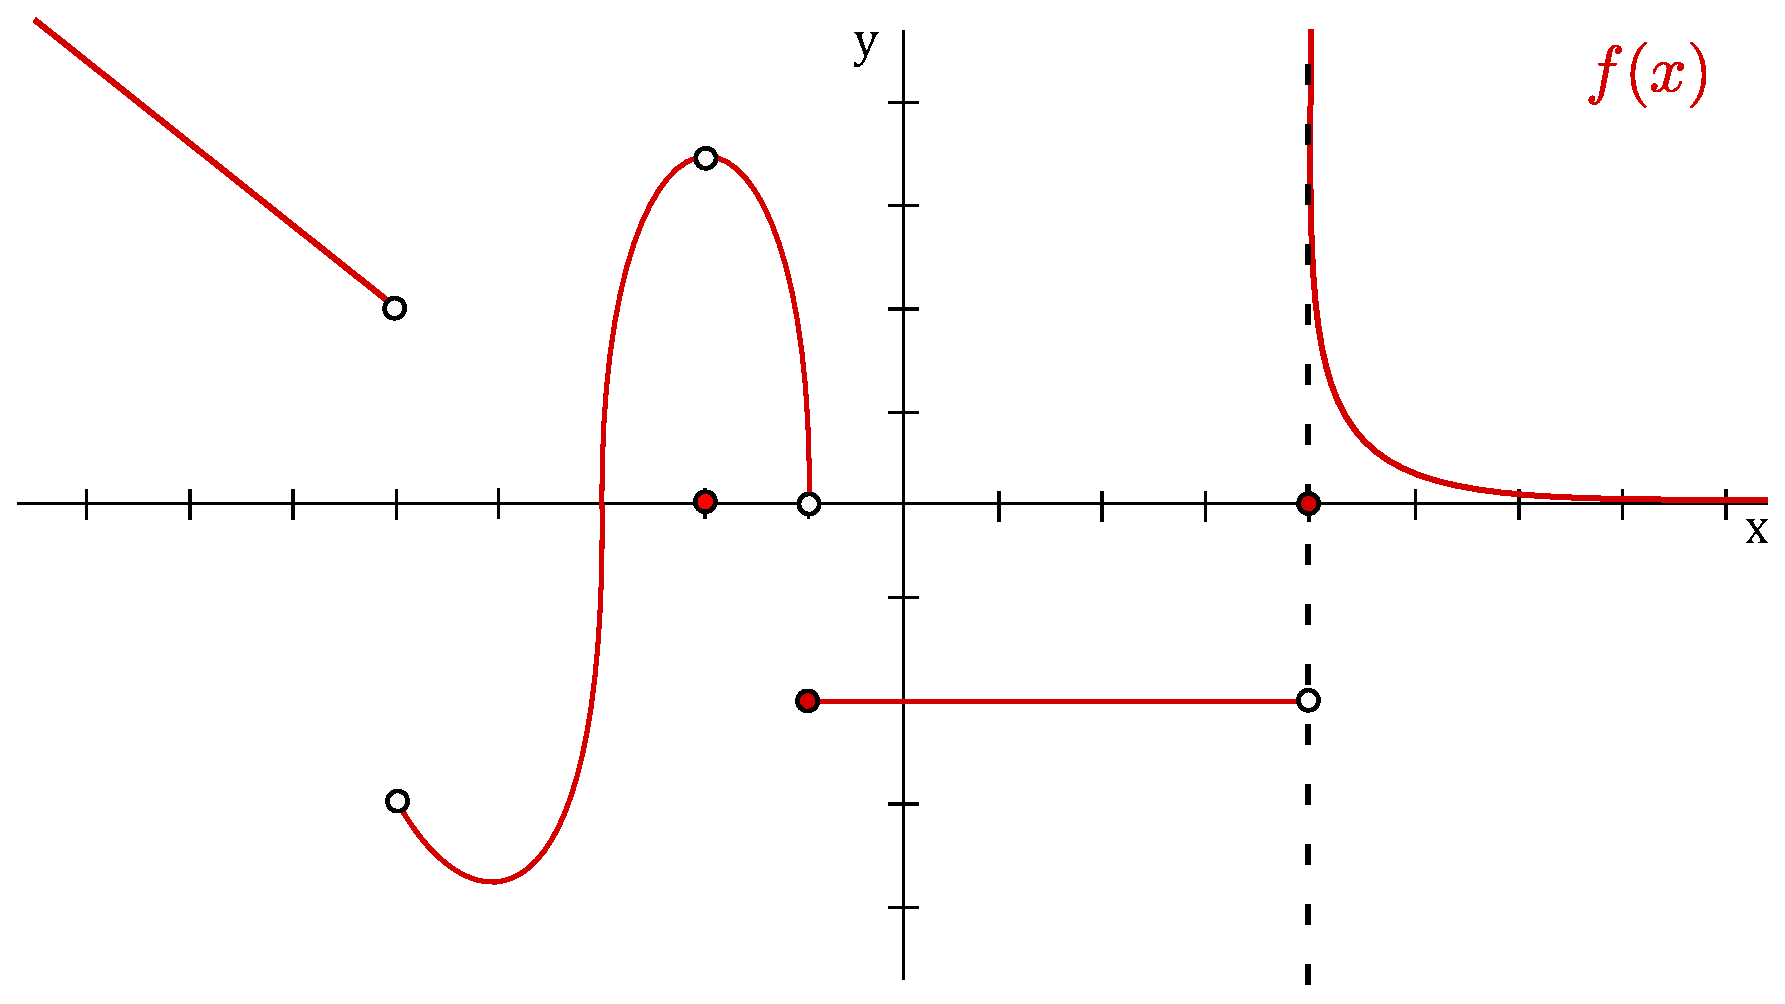
\includegraphics[width=5.3in]{images/limits-graphically}
\caption{A function with discontinuities at $x=-5$, $x=-2$, $x=-1$ and $x=4$. \label{fig:discontgraph}}
\endfigure

We can draw this function without lifting our pencil \ifont{except} at the points $x=-5$, $x=-2$, $x=-1$, and $x=4$.
Thus, $f(x)$ is \ifont{continuous} at every real number \ifont{except} at these four numbers.
At $x=-5$, $x=-2$, $x=-1$, and $x=4$, the function $f(x)$ is \ifont{discontinuous}.

At $x=-2$ we have a \dfont{removable discontinuity} because we could remove this discontinuity simply by redefining $f(-2)$ to be $3.5$.
At $x=-5$ and $x=-1$ we have \dfont{jump discontinuities} because the function jumps from one value to another.
From the right of $x=4$, we have an \dfont{infinite discontinuity} because the function goes off to infinity.

Formally, we say $f(x)$ has a \dfont{removable discontinuity} at $x=a$ if $\lim_{x\to a}f(x)$ exists but is not equal to $f(a)$. Note that we do not require $f(a)$ to be defined in this case, that is, $a$ need not belong to the domain of $f(x)$.

$$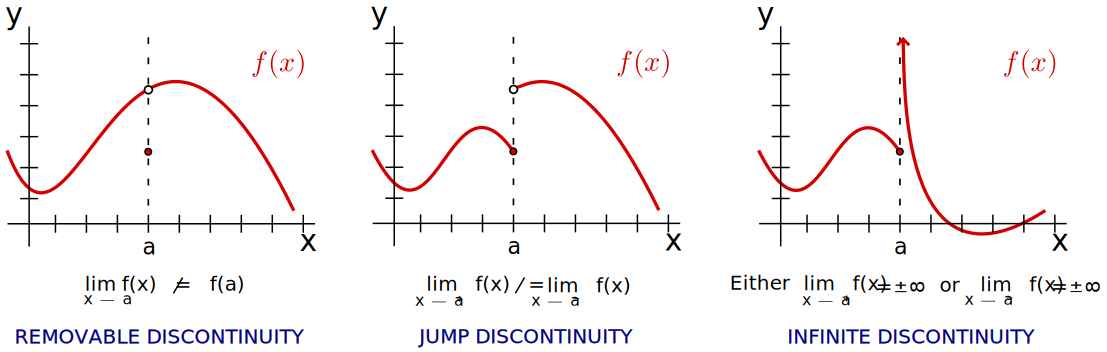
\includegraphics[width=6.4in]{images2/continuity-types-of-discont}$$

\begin{example}{Continuous at a Point}{ContinuousPoint}
	What value of $c$ will make the following function $f(x)$ continuous at $2$?
	$$f(x)=\left\{\begin{array}{cl}
	\ds{\frac{x^2-x-2}{x-2}}&\qquad\mbox{if $x\neq 2$}\\
	\\
	c&\qquad\mbox{if $x=2$}\\\end{array}\right.$$
\end{example}
\begin{solution} 
	In order to be continuous at $2$ we require 
	$$\lim_{x\to 2}f(x)=f(2)$$
	to hold.
	We use the three part definition listed previously to check this.
	
	1. First, $f(2)=c$, and $c$ is some real number. Thus, $f(2)$ is defined.
	
	2. Now, we must evaluate the limit. 
	Rather than computing both one-sided limits, we just compute the limit directly.
	For $x$ close to $2$ (but not equal to $2$) we can replace $f(x)$ with $\frac{x^2-x-2}{x-2}$ to get:
	$$\lim_{x\to 2}f(x)=\lim_{x\to 2}\frac{x^2-x-2}{x-2}=\lim_{x\to 2}\frac{(x-2)(x+1)}{x-2}=\lim_{x\to 2}(x+1)=3.$$
	Therefore the limit exists and equals $3$.
	
	3. Finally, for $f$ to be continuous at $2$, we need that the numbers in the first two items to be equal.
	Therefore, we require $c=3$.
	Thus, when $c=3$, $f(x)$ is continuous at $2$, for any other value of $c$, $f(x)$ is discontinuous at $2$.
\end{solution}


\begin{example}{Finding intervals of continuity}{ex_contint2}{
The \textit{floor function},\index{floor function} $f(x) = \lfloor x \rfloor$, returns the largest integer smaller than the input $x$. (For example, $f(\pi) = \lfloor \pi \rfloor = 3$.) The graph of $f$ in Figure \ref{fig:continuous2} demonstrates why this is often called a ``step function.'' \\

\noindent Give the intervals on which $f$ is continuous.

\mfigure{.7}{A graph of the step function in Example \ref{exa:ex_contint2}.}{fig:continuous2}{\begin{tikzpicture}
\begin{axis}[minor x tick num=1,axis y line=middle,axis x line=middle,ymin=-2.4,ymax=2.4,xmin=-2.4,xmax=3.4,name=myplot]
\addplot [{\colorone},smooth,thick] coordinates {(-2,-2) (-1,-2)};
\addplot [{\colorone},smooth,thick] coordinates {(-1,-1) (0,-1)};
\addplot [{\colorone},smooth,thick] coordinates {(0,0) (1,0)};
\addplot [{\colorone},smooth,thick] coordinates {(1,1) (2,1)};
\addplot [{\colorone},smooth,thick] coordinates {(2,2) (3,2)};
\fill[white,draw=black] (axis cs:-1,-2) circle (1pt);
\fill[black,draw=black] (axis cs:-2,-2) circle (1pt);

\fill[white,draw=black] (axis cs:0,-1) circle (1pt);
\fill[black,draw=black] (axis cs:-1,-1) circle (1pt);

\fill[white,draw=black] (axis cs:1,0) circle (1pt);
\fill[black,draw=black] (axis cs:0,0) circle (1pt);

\fill[white,draw=black] (axis cs:2,1) circle (1pt);
\fill[black,draw=black] (axis cs:1,1) circle (1pt);

\fill[white,draw=black] (axis cs:3,2) circle (1pt);
\fill[black,draw=black] (axis cs:2,2) circle (1pt);
\end{axis}
\node [right] at (myplot.right of origin) {  $x$};
\node [above] at (myplot.above origin) {  $y$};
\end{tikzpicture}}
}
\end{example}


\begin{solution}
{We examine the three criteria for continuity.
		\begin{enumerate}
		\item		The limits $\lim_{x\to c} f(x)$ do not exist at the jumps from one ``step'' to the next, which occur at all integer values of $c$. Therefore the limits exist for all $c$ except when $c$ is an integer.
		\item		The function is defined for all values of $c$.
		\item		The limit $\ds \lim_{x\to c} f(x) = f(c)$ for all values of $c$ where the limit exist, since each step consists of just a line. 
		\end{enumerate}
		We conclude that $f$ is continuous everywhere except at integer values of $c$. So the intervals on which $f$ is continuous are $$\ldots, (-2,-1), (-1,0), (0,1), (1,2), \ldots.$$
}
\end{solution}




		
Our definition of continuity on an interval specifies the interval is an open interval. We can extend the definition of continuity to closed intervals by considering the appropriate one-sided limits at the endpoints.

\begin{definition}{Continuous from the Right and from the Left}{ContinuousRightLeftDefinition}
A function $f$ is \deffont{left continuous at a point $a$} if
\[\ds \lim_{x\to a^-} f(x) = f(a)\]

and \deffont{right continuous at a point $a$} if
\[\ds \lim_{x\to a^+} f(x) = f(a).\]
\end{definition}

If a function $f$ is continuous at $a$, then it is both left and right continuous at $a$.

The above definition regarding left (or right) continuous functions is illustrated with the following figure:
$$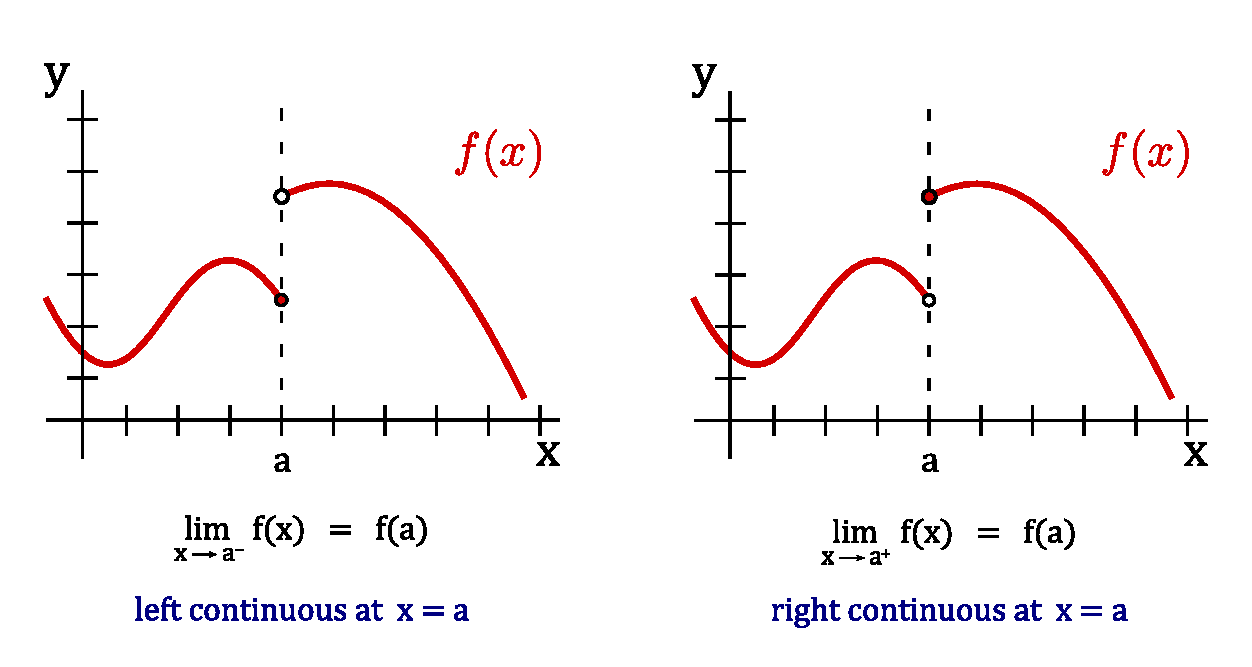
\includegraphics[width=4.7in]{images2/continuity-left-and-right}$$

One-sided limits allows us to extend the definition of continuity to closed intervals. The following definition means a function is continuous on a closed interval if it is continuous in the interior of the interval and possesses the appropriate one-sided continuity at the endpoints of the interval.

\begin{definition}{Continuity on a Closed Interval}{ContinuityClosedIntervalDefinition}
A function $f$ is \deffont{continuous on the closed interval $[a,b]$} if:
\begin{enumerate}
	\item[(i)] it is continuous on the open interval $(a,b)$;
	\item[(ii)] it is left continuous at point $a$:
	\[\ds\lim_{x\to a^-}f(x)=f(a);\]
	and
	\item[(iii)] it is right continuous at point $b$:
	\[\ds\lim_{x\to b^+}f(x)=f(b).\]
\end{enumerate}

\end{definition}

This definition can be extended to continuity on half-open intervals such as $(a,b]$ and $[a,b)$, and unbounded intervals.

\begin{example}{Continuity on Other Intervals}{ContinuityOtherInt}
The function $f(x)=\sqrt{x}$ is continuous on the (closed) interval $[0,\infty)$.

\medskip
The function $f(x)=\sqrt{4-x}$ is continuous on the (closed) interval $(-\infty,4]$.
\end{example}

The continuity of functions is preserved under the operations of addition, subtraction, multiplication and division (in the case that the function in the denominator is nonzero).

\begin{theorem}{Operations of Continuous Functions}{OpsContFunct}
If $f$ and $g$ are continous at $a$, and $c$ is a constant, then the following functions are also \ifont{continuous} at $a$:
\begin{multicols}{2}
\begin{enumerate}[(i)]
\item $f\pm g$; 
\item $cf$; 
\item $fg$; 
\item $f/g$ (provided $g(a)\neq 0$).
\end{enumerate}
\end{multicols}
\end{theorem}

\begin{example}{Determining intervals on which a function is continuous}{ex_cont_funct}{
State the interval(s) on which each of the following functions is continuous.

		\noindent\begin{minipage}{.5\linewidth}
		\begin{enumerate}
		\item		$\ds f(x) = \sqrt{x-1} + \sqrt{5-x}$
		\item		$\ds f(x) = x\sin x$
		\end{enumerate}
		\end{minipage}
		\begin{minipage}{.5\linewidth}
		\begin{enumerate}\addtocounter{enumi}{2}
		\item		$\ds f(x) = \tan x$
		\item		$\ds f(x) = \sqrt{\ln x}$
		\end{enumerate}
		\end{minipage}
}
\end{example}


\begin{solution}
{We examine each in turn.
		\begin{enumerate}
			\item		The square--root terms are continuous on the intervals $[1,\infty)$ and $(-\infty,5]$, respectively. As $f$ is continuous only where each term is continuous, $f$ is continuous on $[1,5]$, the intersection of these two intervals. A graph of $f$ is given in Figure \ref{fig_continuous3}.
			
	\mfigure{.7}{A graph of $f$ in Example \ref{exa:ex_cont_funct}(a).}{fig_continuous3}{\begin{tikzpicture}
	\begin{axis}[minor x tick num=1,axis y line=middle,axis x line=middle,ymin=-.4,ymax=3.2,xmin=-.4,xmax=5.4,name=myplot]
	\addplot [{\colorone},smooth,thick] coordinates {(1.,2.)(1.01,2.0975) (1.02,2.13642) (1.03,2.16569) (1.04,2.18997) (1.05,2.21107) (1.1,2.29107) (1.15,2.34944) (1.2,2.39657) (1.3,2.47126) (1.4,2.52982)
	(1.5,2.57794) (1.6,2.61851) (1.7,2.65325) (1.8,2.68328) (1.9,2.70936)
	(2.,2.73205) (2.1,2.75175) (2.2,2.76877) (2.3,2.78334) (2.4,2.79567) 
	(2.5,2.80588) (2.6,2.8141) (2.7,2.82042) (2.8,2.82488) (2.9,2.82754) 
	(3.,2.82843) (3.1,2.82754) (3.2,2.82488) (3.3,2.82042) (3.4,2.8141) (3.5,2.80588) (3.6,2.79567) (3.7,2.78334) (3.8,2.76877) (3.9,2.75175)(4.,2.73205) (4.1,2.70936) (4.2,2.68328) (4.3,2.65325) (4.4,2.61851)(4.5,2.57794) (4.6,2.52982) (4.7,2.47126) (4.8,2.39657) (4.85,2.34944) (4.9,2.29107) (4.95,2.21107) (4.96,2.18997) (4.97,2.16569) (4.98,2.13642) (4.99,2.0975)(5.,2.)
	};
	%\addplot [{\colorone},smooth] coordinates {(1.,1.) (2,1)};
	%\addplot [{\colorone},smooth] coordinates {(2.,1.) (2.1,1.09) (2.2,1.16) (2.3,1.21) (2.4,1.24) (2.5,1.25)
	%(2.6,1.24) (2.7,1.21) (2.8,1.16) (2.9,1.09) (3.,1.)};
	%\fill[white,draw=black] (axis cs:2,0) circle (1pt);
	\fill[black,draw=black] (axis cs:1,2) circle (1pt);
	\fill[black,draw=black] (axis cs:5,2) circle (1pt);
	%\fill[black,draw=black] (axis cs:3,1) circle (1pt);
	\end{axis}
	\node [right] at (myplot.right of origin) {  $x$};
	\node [above] at (myplot.above origin) {  $y$};
	\end{tikzpicture}}
			\item		The functions $y=x$ and $y=\sin x$ are each continuous everywhere, hence their product is, too.
			\item	 $f(x) = \tan x$ is continuous ``on its domain.'' Its domain includes all real numbers except odd multiples of $\pi/2$. Thus $f(x) = \tan x$ is continuous on $$\ldots \left(-\frac{3\pi}{2},-\frac{\pi}2\right),\ \left(-\frac{\pi}2,\frac{\pi}2\right),\ \left(\frac{\pi}2,\frac{3\pi}2\right),\ldots,$$ or, equivalently, on $D = \{x\in \mathbb{R}\ |\ x\neq n\cdot \frac{\pi}2,\ $n$\ \text{is an odd integer} \}.$
			\item		The domain of $y = \sqrt{x}$ is $[0,\infty)$. The range of $y=\ln x$ is $(-\infty,\infty)$, but if we restrict its domain to $[1,\infty)$ its range is $[0,\infty)$. So restricting $y = \ln x$ to the domain of $[1,\infty)$ restricts its output is $[0,\infty)$, on which $y = \sqrt{x}$ is defined. Thus the domain of $f(x) = \sqrt{\ln x}$ is $[1,\infty)$.
			\end{enumerate}
}
\end{solution}









The next theorem states that the inverse $ f^{-1} $ of a continuous function $ f(x) $ is also continuous. This is not so surprising because the graph of $ f^{-1}(x) $ is a reflection of the graph of $ f(x) $ through the line $ y=x $. If the graph of $ f $ has no "breaks" in it, then neither will the graph of $ f^{-1} $.

\begin{theorem}{Continuity of Inverse Functions}{InvCont}
If $ f(x) $ is continuous on an interval $ I $, with range $ R $, then $ f^{-1} $ is continuous on every interval of the domain $ R $.
\end{theorem}

One consequence of this is that the inverse trigonometric functions are all continuous on their respective domains. Below we list some common functions that are known to be continuous on every interval inside their domains.

\begin{example}{Common Types of Continuous Functions}{CommonContinuousFunctionsList}
\begin{itemize}
	\item	Polynomials (for all $x$), e.g., $y=mx+b$, $y=ax^2+bx+c$.
	\item	Rational functions (except at points $x$ which gives division by zero).
	\item	Root functions $\sqrt[n]{x}$ (for all $x$ if $n$ is odd, and for $x\geq 0$ if $n$ is even).
	\item	Trigonometric functions
	\item	Inverse trigonometric functions
	\item	Exponential funtions
	\item	Logarithmic functions
\end{itemize}
\end{example}

For rational functions with removable discontinuities as a result of a zero, we can define a new function filling in these gaps to create a piecewise function that is continuous everywhere.

Continuous functions are where the \ifont{direct substitution
property} hold. This fact can often be used to compute the limit of a
continuous function.

\begin{example}{Evaluate a Limit}{EvaluateLimit}
Evaluate the following limit:
$\ds\lim_{x\to\pi}\frac{\sqrt{x}+\sin x}{1+x+\cos x}$.
%\vspace{-0.5cm}
\end{example}

\begin{solution} 
We will use a continuity argument to justify that direct substitution can be applied.
By the list above, $\sqrt{x}$, $\sin x$, $1$, $x$ and $\cos x$ are all continuous functions at $\pi$.
Then $\sqrt x+\sin x$ and $1+x+\cos x$ are both continuous at $\pi$.
Finally,
$$\frac{\sqrt{x}+\sin x}{1+x+\cos x}$$
is a continuous function at $\pi$ since $1+\pi+\cos\pi\neq 0$.
Hence, we can directly substitute to get the limit:
$$\lim_{x\to\pi}\frac{\sqrt{x}+\sin x}{1+x+\cos x}=\frac{\sqrt{\pi}+\sin \pi}{1+\pi+\cos \pi}=\frac{\sqrt{\pi}}{\pi}=\frac{1}{\sqrt{\pi}}.$$
\end{solution}

Continuity is also preserved under the composition of functions.

\begin{theorem}{Continuity of Function Composition}{ContinuityFunctionComposition}
If $g$ is continuous at $a$ and $f$ is continuous at $g(a)$, then the composition function $f\circ g$ is continuous at $a$.
\end{theorem}

\begin{example}{Continuity with Composition of Functions}{ContCompositions}
Determine where the following functions is continuous:
\begin{enumerate}[(a)]
	\item	$h(x)=\cos(x^2)$
	\item	$H(x)=\ln(1+\sin(x))$
\end{enumerate}
\end{example}
\begin{solution}
\begin{enumerate}[(a)]
	\item	The functions that make up the composition $h(x)=f(g(x))$
	are $g(x)=x^2$ and $f(x)=\cos(x)$.
	The function $g$ is continuous on $\mathbb{R}$ since it is a polynomial,
	and $f$ is also continuous everywhere. Therefore, $h(x)=(f\circ g)(x)$
	is continuous on $\mathbb{R}$ by Theorem~\ref{thm:ContinuityFunctionComposition}.
	\item	We know from Example~\ref{exa:CommonContinuousFunctionsList}
	that $f(x)=\ln x$ is continuous and $g(x)=1+\sin x$ are continuous. Thus by
	Theorem~\ref{thm:ContinuityFunctionComposition}, $H(x)=f(g(x))$ is continuous
	wherever it is defined. Now $\ln(1+\sin x)$ is defined when $1+\sin x>0$.
	Recall that $-1\leq \sin x\leq 1$, so $1+\sin x>0$ except when $\sin x=-1$,
	which happens when $x=\pm 3\pi/2,\pm 7\pi/2,\ldots$. Therefore, $H$ has discontinuities
	when $x=3\pi n/2$, $n=1,2,3,\ldots$ and is continuous on the intervals between these values.
\end{enumerate}
\end{solution}


%%%%%%%%%%%%%%%%%%%%%%%%%%%%%%%%%%%%%%%%%
\subsection*{Intermediate Value Theorem}
Whether or not an equation \ifont{has} a solution is an important question in mathematics.
Consider the following two questions:

\begin{example}{Motivation for the Intermediate Value Theorem}{Motivation for IVT}\label{MotivationforIVT}
\vspace{-0.5cm}
\begin{enumerate}
	\item Does $e^x+x^2=0$ have a solution?
	\item Does $e^x+x=0$ have a solution?
\end{enumerate}
\end{example}

\begin{solution} 
\begin{enumerate}
	\item	The first question is easy to answer since for any exponential function we know that $a^x>0$, and we also know that whenever you square a number you get a nonnegative answer: $x^2\geq 0$. Hence, $e^x+x^2>0$, and thus, is never equal to zero. Therefore, the first equation has no solution.
	\item	For the second question, it is difficult to see if $e^x+x=0$ has a solution.
	If we tried to solve for $x$, we would run into problems.
	Let's make a table of values to see what kind of values we get (recall that $e\approx 2.7183$):
	$$\begin{array}{c|c}
	x & e^x+x\\
	\hline
	-2 & e^{-2}-2\approx -1.9\\
	-1 & e^{-1}-1\approx -0.6\\
	0 & e^0+0=1\\
	1 & e+1\approx 3.7\\
	\end{array}$$
	Sketching this gives:
	$$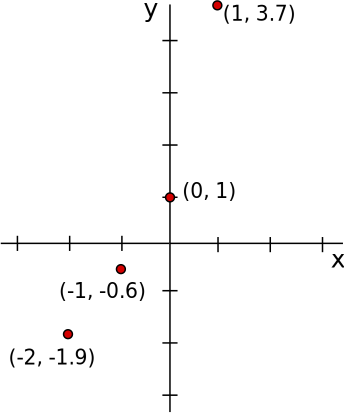
\includegraphics[width=1.9in]{images/ivt1}$$
	Let $f(x)=e^x+x$.
	Notice that if we choose $a=-1$ and $b=0$ then we have $f(a)<0$ and $f(b)>0$.
	A point where the function $f(x)$ crosses the $x$-axis gives a solution to $e^x+x=0$.
	Since $f(x)=e^x+x$ is continuous (both $e^x$ and $x$ are continuous), then the function \ifont{must} cross the $x$-axis somewhere between $-1$ and $0$:
	$$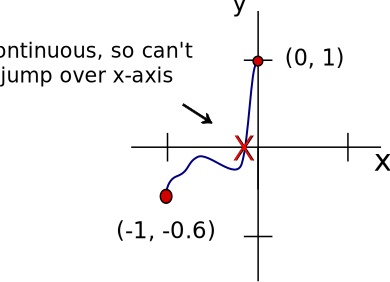
\includegraphics[width=2.2in]{images/ivt2}$$
	Therefore, our equation has a solution.
	
	Note that by looking at smaller and smaller intervals $(a,b)$ with $f(a)<0$ and $f(b)>0$, we can get a better and better approximation for a solution to $e^x+x=0$.
	For example, taking the interval $(-0.4,-0.6)$ gives $f(-0.4)<0$ and $f(-0.6)>0$, thus, there is a solution to $f(x)=0$ between $-0.4$ and $-0.6$.
	It turns out that the solution to $e^x+x=0$ is $x\approx -0.56714$.
\end{enumerate}
\end{solution}

We now generalize the argument used in the previous example.
In that example we had a continuous function that went from negative to positive and hence, had to cross the $x$-axis at some point.
In fact, we don't need to use the $x$-axis, any line $y=N$ will work so long as the function is continuous and below the line $y=N$ at some point and above the line $y=N$ at another point.
This is known as the Intermediate Values Theorem and it is formally stated as follows:

\begin{theorem}{Intermediate Value Theorem}{IntermediateValueTheorem}
If $f$ is continuous on the interval
$[a,b]$ and $N$ is between $f(a)$ and $f(b)$, where $f(a)\neq f(b)$,
then there is a number $c$ in $(a,b)$ such that $f(c)=N$. 
\end{theorem}

The Intermediate Value Theorem guarantees that if $f(x)$ is continuous and $f(a)<N<f(b)$, the line $y=N$ intersects the function at some point $x=c$. Such a number $c$ is between $a$ and $b$ and has the property that $f(c)=N$ (see Figure \ref{fig-ivt}(a)).
We can also think of the theorem as saying if we draw the line $y=N$ between the lines $y=f(a)$ and $y=f(b)$, then the function cannot jump over the line $y=N$.
On the other hand, if $f(x)$ is \ifont{not} continuous, then the theorem may \ifont{not} hold.
See Figure \ref{fig-ivt}(b) where there is no number $c$ in $(a,b)$ such that $f(c)=N$.
Finally, we remark that there may be multiple choices for $c$ (i.e., lots of numbers between $a$ and $b$ with $y$-coordinate $N$). See Figure \ref{fig-ivt}(c) for such an example.
\begin{figure}[!ht]
$$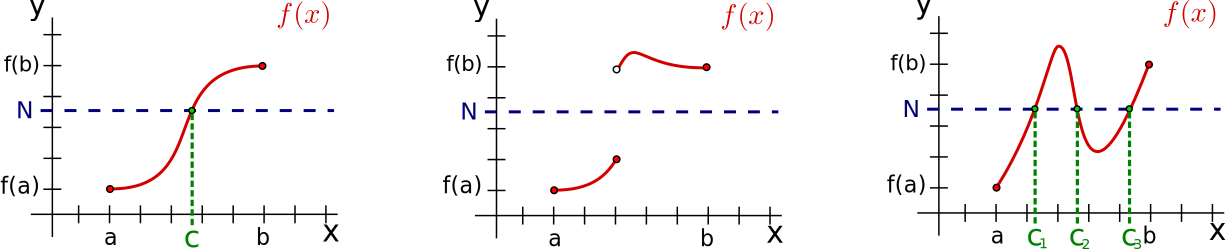
\includegraphics[width=6in]{images/ivt3}$$
\caption{(a) A continuous function where IVT holds for a single value $c$.
(b) A discontinuous function where IVT fails to hold. 
(c) A continuous function where IVT holds for multiple values in $(a,b)$. \label{fig-ivt}}
\end{figure}

The Intermediate Value Theorem is most frequently used for $N=0$.

\begin{example}{Intermediate Value Theorem}{IntermediateValueTheorem}
Show that there is a solution of $\sqrt[3]{x}+x=1$ in the interval $(0,8)$.
\end{example}

\begin{solution} 
Let $f(x)=\sqrt[3]{x}+x-1$, $N=0$, $a=0$, and $b=8$.
Since $\sqrt[3]{x}$, $x$ and $-1$ are continuous on $\mathbb{R}$, and the sum of continuous functions is again continuous, we have that $f(x)$ is continuous on $\mathbb{R}$, thus in particular, $f(x)$ is continuous on $[0,8]$.
We have $f(a)=f(0)=\sqrt[3]{0}+0-1=-1$ and $f(b)=f(8)=\sqrt[3]{8}+8-1=9$.
Thus $N=0$ lies between $f(a)=-1$ and $f(b)=9$, so the conditions of the Intermediate Value Theorem are satisfied.
So, there exists a number $c$ in $(0,8)$ such that $f(c)=0$.
This means that $c$ satisfies $\sqrt[3]{c}+c-1=0$, in otherwords, is a solution for the equation given.

Alternatively we can let $f(x)=\sqrt[3]{x}+x$, $N=1$, $a=0$ and $b=8$.
Then as before $f(x)$ is the sum of two continuous functions, so is also continuous everywhere, in particular, continuous on the interval $[0,8]$.
We have $f(a)=f(0)=\sqrt[3]{0}+0=0$ and $f(b)=f(8)=\sqrt[3]{8}+8=10$.
Thus $N=1$ lies between $f(a)=0$ and $f(b)=10$, so the conditions of the Intermediate Value Theorem are satisfied.
So, there exists a number $c$ in $(0,8)$ such that $f(c)=1$.
This means that $c$ satisfies $\sqrt[3]{c}+c=1$, in otherwords, is a solution for the equation given.
\end{solution}

\begin{example}{Roots of Function}{RootsFunction}
Explain why the function $\ds f=x^3 + 3x^2+x-2$ has a root between 0
and 1.
\end{example}

\begin{solution}
By theorem~\ref{thm:PropertiesLimits}, $f$ is continuous.
Since $f(0)=-2$ and $f(1)=3$, and $0$ is between $-2$ and $3$, there
is a $c\in(0,1)$ such that $f(c)=0$.
\end{solution}




One important application of the Intermediate Value Theorem is root finding. Given a function $f$, we are often interested in finding values of $x$ where $f(x) = 0$. These roots may be very difficult to find exactly. Good approximations can be found through successive applications of this theorem. Suppose through direct computation we find that $f(a) <0 $ and $f(b)>0$, where $a<b$. The Intermediate Value Theorem states that there is a $c$ in $[a,b]$ such that $f(c) = 0$. The theorem does not give us any clue as to where that value is in the interval $[a,b]$, just that it exists. 

There is a technique that produces a good approximation of $c$. Let $d$ be the midpoint of the interval $[a,b]$ and consider $f(d)$. There are three possibilities:
	\begin{enumerate} 
	\item		$f(d) = 0$ -- we got lucky and stumbled on the actual value. We stop as we found a root.
	\item		$f(d) <0$ Then we know there is a root of $f$ on the interval $[d,b]$ -- we have halved the size of our interval, hence are closer to a good approximation of the root.
	\item		$f(d) >0$ Then we know there is a root of $f$ on the interval $[a,d]$ -- again,we have halved the size of our interval, hence are closer to a good approximation of the root.
	\end{enumerate}

\enlargethispage{2\baselineskip}	
Successively applying this technique is called the \textit{Bisection Method} \index{Bisection Method} of root finding. We continue until the interval is sufficiently small. We demonstrate this in the following example.\\

\begin{example}{Using the Bisection Method}{ex_bisect_method}{
Approximate the root of $f(x) = x-\cos x$, accurate to three places after the decimal.}
\end{example}


\begin{solution}
{Consider the graph of $f(x) = x-\cos x$, shown in Figure \ref{fig:xminuscosx}. It is clear that the graph crosses the $x$-axis somewhere near $x=0.8$. To start the Bisection Method, pick an interval that contains $0.8$. We choose $[0.7,0.9]$. Note that all we care about are signs of $f(x)$, not their actual value, so this is all we display.

\mfigure{.8}{Graphing a root of $f(x) = x-\cos x$.}{fig:xminuscosx}{\begin{tikzpicture}
\begin{axis}[minor x tick num=4,axis y line=middle,axis x line=middle,ymin=-1.1,ymax=.7,xmin=-.05,xmax=1.07,name=myplot]
\addplot [{\colorone},smooth,thick] coordinates {(0.,-1.) (0.05,-0.94875) (0.1,-0.895004) (0.15,-0.838771)(0.2,-0.780067) (0.25,-0.718912) (0.3,-0.655336) (0.35,-0.589373)(0.4,-0.521061) (0.45,-0.450447) (0.5,-0.377583) (0.55,-0.302525)(0.6,-0.225336) (0.65,-0.146084)(0.7,-0.0648422) (0.71,-0.0483619) (0.72,-0.0318057)(0.73,-0.0151744) (0.74,0.00153144) (0.75,0.0183111) (0.76,0.035164)(0.77,0.0520893) (0.78,0.0690865) (0.79,0.0861547) (0.8,0.103293)(0.85,0.190017) (0.9,0.27839) (0.95,0.368317) (1.,0.459698)
};
\end{axis}
\node [right] at (myplot.right of origin) {  $x$};
\node [above] at (myplot.above origin) { $y$};
%\spy [{\colortwo}] on (1,1) in node at (1.5,-2);
\end{tikzpicture}}

		\begin{description}
		\item [Iteration 1:] $f(0.7) < 0$, $f(0.9) > 0$, and $f(0.8) >0$. So replace $0.9$ with $0.8$ and repeat.
		\item	[Iteration 2:]	$f(0.7)<0$, $f(0.8) > 0$, and at the midpoint, $0.75$, we have $f(0.75) >0 $. So replace $0.8$ with $0.75$ and repeat. Note that we don't need to continue to check the endpoints, just the midpoint. Thus we put the rest of the iterations in Table \ref{table:rootfinding}.
		\end{description}
		
\mtable{.5}{Iterations of the Bisection Method of Root Finding}{table:rootfinding}%
			{ \noindent \begin{tabular}{ccc}
			Iteration \# & Interval & Midpoint Sign \\ \hline
			1		& $[0.7,0.9]$ & $f(0.8) >0$ \\
			2 & $[0.7,0.8] $ & $f(0.75) >0$ \\
			3 & $[0.7,0.75]$ & $f(0.725)<0$\\
			4 & $[0.725,0.75]$ & $f(0.7375)<0$\\
			5 & $[0.7375,0.75]$ & $f(0.7438)>0$\\
			6 & $[0.7375,0.7438]$ & $f(0.7407)>0$\\
			7 & $[0.7375,0.7407]$ & $f(0.7391)>0$\\
			8 & $[0.7375,0.7391]$ & $f(0.7383)<0$\\
			9 & $[0.7383,0.7391]$ & $f(0.7387)<0$\\
			10 & $[0.7387,0.7391]$ & $f(0.7389)<0$\\
			11 & $[0.7389,0.7391]$ & $f(0.7390)<0$\\
			12 & $[0.7390,0.7391]$ &   \\
			\end{tabular}
			}%
			
Notice that in the 12$^\text{th}$ iteration we have the endpoints of the interval each starting with $0.739$. Thus we have narrowed the zero down to an accuracy of the first three places after the decimal. Using a computer, we have 
$$ f(0.7390) = -0.00014, \quad f(0.7391) = 0.000024.$$ Either endpoint of the interval gives a good approximation of where $f$ is 0. The Intermediate Value Theorem states that the actual zero is still within this interval. While we do not know its exact value, we know it starts with $0.739$. 

This type of exercise is rarely done by hand. Rather, it is simple to program a computer to run such an algorithm and stop when the endpoints differ by a preset small amount. One of the authors did write such a program and found the zero of $f$, accurate to 10 places after the decimal, to be 0.7390851332. While it took a few minutes to write the program, it took less than a thousandth of a second for the program to run the necessary 35 iterations. In less than 8 hundredths of a second, the zero was calculated to 100 decimal places (with less than 200 iterations).
}\\
\end{solution}




It is a simple matter to extend the Bisection Method to solve problems similar to ``Find $x$, where $f(x) = 0$.'' For instance, we can find $x$, where $f(x) = 1$. %This may seem obvious, but to many it is not. 
It actually works very well to define a new function $g$ where $g(x) = f(x) - 1$. Then use the Bisection Method to solve $g(x)=0$.  
 

Similarly, given two functions $f$ and $g$, we can use the Bisection Method to solve $f(x) = g(x)$. Once again, create a new function $h$ where $h(x) = f(x)-g(x)$ and solve $h(x) = 0$. 

In Section \ref{sec:Newton} another equation solving method will be introduced, called Newton's Method. In many cases, Newton's Method is much faster. It relies on more advanced mathematics, though, so we will wait before introducing it. 

This section formally defined what it means to be a continuous function. ``Most'' functions that we deal with are continuous, so often it feels odd to have to formally define this concept. Regardless, it is important, and forms the basis of the next chapter.

In the next section we examine one more aspect of limits: limits that involve infinity.


%This example also points the way to a simple method for  approximating
%roots.
%
%\begin{example}{Approximating Roots}{ApproximatingRoots}
%Approximate the root of the previous example  to one decimal
%place.
%\end{example}
%
%\begin{solution}
%If we compute $f(0.1)$, $f(0.2)$, and so on, we find that 
%$f(0.6)<0$ and $f(0.7)>0$, so by the Intermediate Value Theorem, $f$
%has a root between $0.6$ and $0.7$. Repeating the process with
%$f(0.61)$, $f(0.62)$, and so on, we find that
%$f(0.61)<0$ and $f(0.62)>0$, so $f$ has a root between
%$0.61$ and $0.62$, and the root is $0.6$ rounded to one decimal place.
%\end{solution}


%%%%%%%%%%%%%%%%%%%%%%%%%%%%%%%%%%%%%%%%%
\Opensolutionfile{solutions}[ex]
\section*{Exercises for \ref{sec:Continuity}}



\begin{enumialphparenastyle}


% % % % % % % % % % %
\begin{ex}
Concepts.
\begin{enumerate}

 
\item {Given functions $f$ and $g$ on an interval $I$, how can the Bisection Method be used to find a value $c$ where $f(c) = g(c)$?}

\item {What is a ``root'' of a function?}

\item {In your own words, describe what the Intermediate Value Theorem states.}


\item {In your own words, describe what it means for a function to be continuous.}
\item {T/F: The sum of continuous functions is also continuous.}
\item {T/F: If $f$ is continuous on $[0,1)$ and $[1,2)$, then $f$ is continuous on $[0,2)$.}

\item {T/F: If $f$ is continuous on $[a,b]$, then $\ds\lim_{x\to a^-}f(x) = f(a)$.}

\item {T/F: If $f$ is continuous at $c$, then $\ds \lim_{x\to c^+}f(x) = f(c)$.}

\item {T/F: If $f$ is continuous at $c$, then $\ds \lim_{x\to c}f(x)$ exists.}

\item {T/F:	If $f$ is defined on an open interval containing $c$, and $\ds \lim_{x\to c}f(x)$ exists, then $f$ is continuous at $c$.
}

\end{enumerate}

\begin{sol}
\begin{enumerate}
\item {Consider the function $h(x) = g(x) - f(x)$, and use the Bisection Method to find a root of $h$.}
\item {A root of a function $f$ is a value $c$ such that $f(c)=0$.}
\item {Answers will vary.}

\item {Answers will vary.}
\item {T}
\item {F}
\item {F}
\item {T}
\item {T}
\item {F}
\end{enumerate}
\end{sol}

\end{ex}
% % % % % % % % % % % %


% % % % % % % % % % %
\begin{ex}

In the following exercises a graph of a function $f$ is given along with a value $a$. Determine if $f$ is continuous at $a$; if it is not, state why it is not.
\begin{multicols}{2}
\begin{enumerate}
\item $ a=1 $ 

\begin{tikzpicture}
\begin{axis}[ %width=\marginparwidth+25pt,tick label style={font=\scriptsize},
axis y line=middle,axis x line=middle,name=myplot,%
%			xtick={-2,-1,1,2,3},% 
%			ytick={-6,-4,-2,0,2,4,6},
%			minor y tick num=1,
%			extra y ticks={-5,-3,...,7},%
			ymin=-.1,ymax=2.1,%
			xmin=-.1,xmax=2.1%
]

\addplot [thick,{\colorone}] coordinates {(0.,1) (1,2)};
\addplot [{\colorone},smooth,thick,domain=1:2] {2*(x-2)^2};

\fill[black,draw=black] (axis cs:0,1) circle (1.5pt);
\fill[white,draw=black] (axis cs:1,2) circle (1.5pt);
\fill[black,draw=black] (axis cs:1,1) circle (1.5pt);
\fill[black,draw=black] (axis cs:2,0) circle (1.5pt);
\end{axis}
\node [right] at (myplot.right of origin) {\scriptsize $x$};
\node [above] at (myplot.above origin) {\scriptsize $y$};
\end{tikzpicture}
\item $ a=1 $

\begin{tikzpicture}
\begin{axis}[ %width=\marginparwidth+25pt,tick label style={font=\scriptsize},
axis y line=middle,axis x line=middle,name=myplot,%
%			xtick={-2,-1,1,2,3},% 
%			ytick={-6,-4,-2,0,2,4,6},
%			minor y tick num=1,
%			extra y ticks={-5,-3,...,7},%
			ymin=-.1,ymax=2.1,%
			xmin=-.1,xmax=2.1%
]

\addplot [thick,{\colorone}] coordinates {(0.,0) (1,1)};
\addplot [{\colorone},thick] coordinates {(1,2) (2,0)};

\fill[black,draw=black] (axis cs:0,0) circle (1.5pt);
\fill[white,draw=black] (axis cs:1,1) circle (1.5pt);
\fill[black,draw=black] (axis cs:1,2) circle (1.5pt);
\fill[black,draw=black] (axis cs:2,0) circle (1.5pt);
\end{axis}
\node [right] at (myplot.right of origin) {\scriptsize $x$};
\node [above] at (myplot.above origin) {\scriptsize $y$};
\end{tikzpicture}
\item $ a=1 $

\begin{tikzpicture}
\begin{axis}[ %width=\marginparwidth+25pt,tick label style={font=\scriptsize},
axis y line=middle,axis x line=middle,name=myplot,%
%			xtick={-2,-1,1,2,3},% 
%			ytick={-6,-4,-2,0,2,4,6},
%			minor y tick num=1,
%			extra y ticks={-5,-3,...,7},%
			ymin=-.1,ymax=2.1,%
			xmin=-.1,xmax=2.1%
]

%\addplot [thick,{\colorone},smooth,domain=0:.9] {1/(x-1)^2};
%\addplot [{\colorone},thick,smooth,domain=1.1:2] {1/(x-1)^2};
\draw [thick,{\colorone}] (axis cs:0,0) parabola (axis cs:1,3);
\draw [thick,{\colorone}] (axis cs:2,0) parabola (axis cs:1,3);
\draw [{\colorone},dashed] (axis cs: 1,2.1) -- (axis cs:1,-.1);

\fill[black,draw=black] (axis cs:0,0) circle (1.5pt);
%\fill[white,draw=black] (axis cs:1,1) circle (1.5pt);
%\fill[black,draw=black] (axis cs:1,2) circle (1.5pt);
\fill[black,draw=black] (axis cs:2,0) circle (1.5pt);
\end{axis}
\node [right] at (myplot.right of origin) {\scriptsize $x$};
\node [above] at (myplot.above origin) {\scriptsize $y$};
\end{tikzpicture}

\item $ a=0 $ 

\begin{tikzpicture}
\begin{axis}[ %width=\marginparwidth+25pt,tick label style={font=\scriptsize},
axis y line=middle,axis x line=middle,name=myplot,%
%			xtick={-2,-1,1,2,3},% 
%			ytick={-6,-4,-2,0,2,4,6},
%			minor y tick num=1,
%			extra y ticks={-5,-3,...,7},%
			ymin=-.1,ymax=2.1,%
			xmin=-.1,xmax=2.1%
]

%\addplot [thick,{\colorone},smooth,domain=0:.9] {1/(x-1)^2};
%\addplot [{\colorone},thick,smooth,domain=1.1:2] {1/(x-1)^2};
\draw [thick,{\colorone}] (axis cs:1,0) parabola (axis cs:2,2);
\draw [thick,{\colorone}] (axis cs:0,1) -- (axis cs:1,2);

\fill[black,draw=black] (axis cs:0,1) circle (1.5pt);
\fill[white,draw=black] (axis cs:1,2) circle (1.5pt);
\fill[black,draw=black] (axis cs:1,1) circle (1.5pt);
\fill[black,draw=black] (axis cs:2,2) circle (1.5pt);
\fill[white,draw=black] (axis cs:1,0) circle (1.5pt);
\end{axis}
\node [right] at (myplot.right of origin) {\scriptsize $x$};
\node [above] at (myplot.above origin) {\scriptsize $y$};
\end{tikzpicture}
\item $ a=1 $ 

\begin{tikzpicture}
\begin{axis}[ %width=\marginparwidth+25pt,tick label style={font=\scriptsize},
axis y line=middle,axis x line=middle,name=myplot,%
%			xtick={-2,-1,1,2,3},% 
%			ytick={-6,-4,-2,0,2,4,6},
%			minor y tick num=1,
%			extra y ticks={-5,-3,...,7},%
			ymin=-.1,ymax=2.1,%
			xmin=-.1,xmax=2.1%
]

%\addplot [thick,{\colorone},smooth,domain=0:.9] {1/(x-1)^2};
%\addplot [{\colorone},thick,smooth,domain=1.1:2] {1/(x-1)^2};
\draw [thick,{\colorone}] (axis cs:1,2) parabola (axis cs:0,0);
\draw [thick,{\colorone}] (axis cs:1,2) -- (axis cs:2,0);

\fill[black,draw=black] (axis cs:0,0) circle (1.5pt);
\fill[black,draw=black] (axis cs:1,2) circle (1.5pt);
\fill[black,draw=black] (axis cs:2,0) circle (1.5pt);
%\fill[black,draw=black] (axis cs:2,2) circle (1.5pt);
%\fill[white,draw=black] (axis cs:1,0) circle (1.5pt);
\end{axis}
\node [right] at (myplot.right of origin) {\scriptsize $x$};
\node [above] at (myplot.above origin) {\scriptsize $y$};
\end{tikzpicture}
\item $ a=4 $ 

 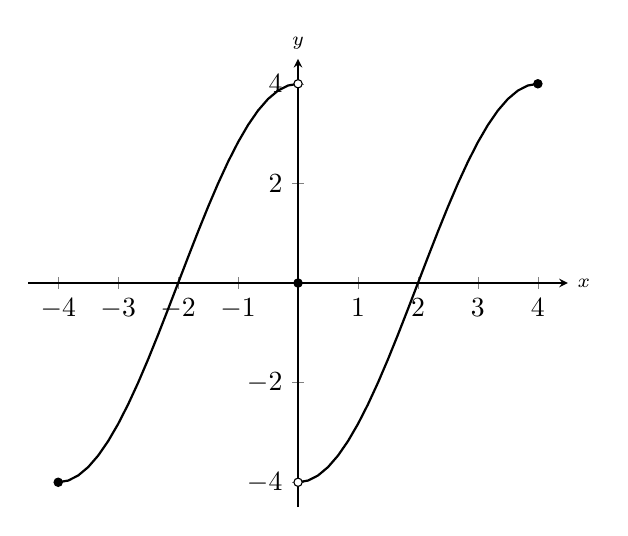
\begin{tikzpicture}
\begin{axis}[ %width=\marginparwidth+25pt,tick label style={font=\scriptsize},
axis y line=middle,axis x line=middle,name=myplot,%
			xtick={-4,...,-1,1,2,...,4},% 
%			ytick={-6,-4,-2,0,2,4,6},
%			minor y tick num=1,
%			extra y ticks={-5,-3,...,7},%
			ymin=-4.5,ymax=4.5,%
			xmin=-4.5,xmax=4.5%
]

%\addplot [thick,{\colorone},smooth,domain=0:.9] {1/(x-1)^2};
%\addplot [{\colorone},thick,smooth,domain=1.1:2] {1/(x-1)^2};
\addplot [thick,{\colorone},domain=-4:0] {4*cos(deg(x)*3.14159/4};
\addplot [thick,{\colorone},domain=0:4]  {-4*cos(deg(x)*3.14159/4};
%
\fill[black,draw=black] (axis cs:0,0) circle (1.5pt);
\fill[white,draw=black] (axis cs:0,4) circle (1.5pt);
\fill[black,draw=black] (axis cs:-4,-4) circle (1.5pt);
\fill[black,draw=black] (axis cs:4,4) circle (1.5pt);
\fill[white,draw=black] (axis cs:0,-4) circle (1.5pt);
\end{axis}
\node [right] at (myplot.right of origin) {\scriptsize $x$};
\node [above] at (myplot.above origin) {\scriptsize $y$};
\end{tikzpicture}

\item \begin{enumerate}
\item		$a = -2$
\item		$a=0$
\item		$a=2$
\end{enumerate}

 \begin{tikzpicture}
\begin{axis}[ %width=\marginparwidth+25pt,tick label style={font=\scriptsize},
axis y line=middle,axis x line=middle,name=myplot,%
			xtick={-4,...,-1,1,2,...,4},% 
%			ytick={-6,-4,-2,0,2,4,6},
%			minor y tick num=1,
%			extra y ticks={-5,-3,...,7},%
			ymin=-4.5,ymax=4.5,%
			xmin=-4.5,xmax=4.5%
]

%\addplot [thick,{\colorone},smooth,domain=0:.9] {1/(x-1)^2};
%\addplot [{\colorone},thick,smooth,domain=1.1:2] {1/(x-1)^2};
\addplot [thick,{\colorone}] coordinates {(-4,0) (-2,2) (0,0) (2,2) (4,0)}; 
%\addplot [thick,{\colorone},domain=0:4]  {-4*cos(deg(x)*3.14159/4};
%
\fill[black,draw=black] (axis cs:0,0) circle (1.5pt);
\fill[black,draw=black] (axis cs:-4,0) circle (1.5pt);
\fill[black,draw=black] (axis cs:-2,0) circle (1.5pt);
\fill[white,draw=black] (axis cs:-2,2) circle (1.5pt);
\fill[white,draw=black] (axis cs:2,2) circle (1.5pt);
\fill[black,draw=black] (axis cs:4,0) circle (1.5pt);
\end{axis}
\node [right] at (myplot.right of origin) {\scriptsize $x$};
\node [above] at (myplot.above origin) {\scriptsize $y$};
\end{tikzpicture}



\item $ a=3 $

\begin{tikzpicture}
\begin{axis}[ %width=\marginparwidth+25pt,tick label style={font=\scriptsize},
axis y line=middle,axis x line=middle,name=myplot,%
			xtick={-4,...,-1,1,2,...,4},% 
%			ytick={-6,-4,-2,0,2,4,6},
%			minor y tick num=1,
%			extra y ticks={-5,-3,...,7},%
			ymin=-4.5,ymax=4.5,%
			xmin=-4.5,xmax=4.5%
]
\draw [thick,{\colorone}] (axis cs:-4,-4) -- (axis cs:-3,-4);
\draw [thick,{\colorone}] (axis cs:-3,-3) -- (axis cs:-2,-3);
\draw [thick,{\colorone}] (axis cs:-2,-2) -- (axis cs:-1,-2);
\draw [thick,{\colorone}] (axis cs:-1,-1) -- (axis cs:0,-1);
\draw [thick,{\colorone}] (axis cs:0,0) -- (axis cs:1,0);
\draw [thick,{\colorone}] (axis cs:1,1) -- (axis cs:2,1);
\draw [thick,{\colorone}] (axis cs:2,2) -- (axis cs:3,2);
\draw [thick,{\colorone}] (axis cs:3,3) -- (axis cs:4,3);

%
\fill[black,draw=black] (axis cs:-4,-4) circle (1.5pt);
\fill[white,draw=black] (axis cs:-3,-4) circle (1.5pt);
\fill[black,draw=black] (axis cs:-3,-3) circle (1.5pt);
\fill[white,draw=black] (axis cs:-2,-3) circle (1.5pt);
\fill[black,draw=black] (axis cs:-2,-2) circle (1.5pt);
\fill[white,draw=black] (axis cs:-1,-2) circle (1.5pt);
\fill[black,draw=black] (axis cs:-1,-1) circle (1.5pt);
\fill[white,draw=black] (axis cs:0,-1) circle (1.5pt);
\fill[black,draw=black] (axis cs:0,0) circle (1.5pt);
\fill[white,draw=black] (axis cs:1,0) circle (1.5pt);
\fill[black,draw=black] (axis cs:1,1) circle (1.5pt);
\fill[white,draw=black] (axis cs:2,1) circle (1.5pt);
\fill[black,draw=black] (axis cs:2,2) circle (1.5pt);
\fill[white,draw=black] (axis cs:3,2) circle (1.5pt);
\fill[black,draw=black] (axis cs:3,3) circle (1.5pt);
\fill[white,draw=black] (axis cs:4,3) circle (1.5pt);
\end{axis}
\node [right] at (myplot.right of origin) {\scriptsize $x$};
\node [above] at (myplot.above origin) {\scriptsize $y$};
\end{tikzpicture}
\end{enumerate}

\begin{sol}
\begin{enumerate}
\item {No; $\ds \lim_{x\to 1} f(x) = 2$, while $f(1) = 1$.}
\item {No; $\ds \lim_{x\to 1} f(x)$ does not exist.}
\item {No; $f(1)$ does not exist.}
\item {Yes}
\item {Yes}
\item {Yes}
\item {\begin{enumerate}
\item		No; $\ds \lim_{x\to -2}f(x) \neq f(-2)$
\item		Yes
\item		No; $f(2)$ is not defined.
\end{enumerate}
}
\item No.
\end{enumerate}
\end{sol}

\end{multicols}
\end{ex}
% % % % % % % % % % % %

% % % % % % % % % % %
\begin{ex}
Determine if $f$ is continuous at the indicated values. If not, explain why.
\begin{enumerate}
\item {$\ds f(x) = \left\{\begin{array}{ccc} 
1		& & x=0\\
\frac{\sin x}{x} & & x>0
\end{array}\right.
$
\begin{enumerate}
\item		$x=0$
\item		$x=\pi$
\end{enumerate}
}

\item {$\ds f(x) = \left\{\begin{array}{ccc} 
x^3-x		& & x<1\\
x-2 & & x\geq 1
\end{array}\right.
$
\begin{enumerate}
\item		$x=0$
\item		$x=1$
\end{enumerate}
}

\item {$\ds f(x) = \left\{\begin{array}{ccc} 
\frac{x^2+5x+4}{x^2+3x+2}		& &  x\neq -1\\
3 & & x=-1
\end{array}\right.
$
\begin{enumerate}
\item		$x=-1$
\item		$x=10$
\end{enumerate}
}

\item {$\ds f(x) = \left\{\begin{array}{ccc}
\frac{x^2-64}{x^2-11 x+24}		& &  x\neq 8\\
5 & & x=8
\end{array}\right.
$
\begin{enumerate}
\item		$x=0$
\item		$x=8$
\end{enumerate}
}

\end{enumerate}

\begin{sol}
\begin{enumerate}
\item {\begin{enumerate}
\item		Yes
\item		Yes
\end{enumerate}
}
\item {\begin{enumerate}
\item		Yes
\item		No; the left and right hand limits at 1 are not equal.
\end{enumerate}
}
\item {\begin{enumerate}
\item		Yes
\item		Yes
\end{enumerate}
}
\item {\begin{enumerate}
\item		Yes
\item		No. $\lim_{x\to 8} f(x) = 16/5 \neq f(8) = 5$.
\end{enumerate}
}
\end{enumerate}
\end{sol}

\end{ex}
% % % % % % % % % % % %

% % % % % % % % % % %
\begin{ex}
Give the intervals on which the given function is continuous.
\begin{enumerate}

\item {$f(x) = x^2-3x+9$
}

\item {$\ds g(x) = \sqrt{x^2-4}$
}

\item {$\ds h(k) = \sqrt{1-k}+\sqrt{k+1}$
}

\item {$\ds f(t) = \sqrt{5t^2-30}$
}


\item {$\ds g(t) = \frac{1}{\sqrt{1-t^2}}$
}

\item {$\ds g(x) = \frac{1}{1+x^2}$
}

\item {$\ds f(x) = e^x$
}

\item {$\ds g(s) = \ln s$
}

\item {$\ds h(t) = \cos t$
}

\item {$\ds f(k) = \sqrt{1-e^k}$
}
\item {$\ds f(x) = \sin(e^x+x^2)$
}
\end{enumerate}

\begin{sol}
\begin{enumerate}
\item {$(-\infty,\infty)$
}
\item {$(-\infty,-2]\cup [2,\infty)$
}
\item {$[-1,1]$
}
\item {$(-\infty,-\sqrt{6}]\cup [\sqrt{6},\infty)$
}
\item {$(-1,1)$
}
\item {$(-\infty,\infty)$
}
\item {$(-\infty,\infty)$
}
\item {$(0,\infty)$
}
\item {$(-\infty,\infty)$
}
\item 
{$(-\infty,0]$
}
\item 
{$(-\infty,\infty)$
} 
\end{enumerate}
\end{sol}

\end{ex}
% % % % % % % % % % % %



%%%%%%%%%%
\begin{ex} 
Consider the function 
$$h(x) = \left\{
\begin{array}{rl}
2x-3, & \mbox{if $x<1$,}\\
0, & \mbox{if $x\geq 1$.}\\
\end{array}\right.$$

Show that it is continuous at the point $x=0$.  Is $h$ a continuous function?
\end{ex}

%%%%%%%%%%
\begin{ex} 
Find the values of $a$ that make the function $f(x)$ continuous for all real numbers.
$$f(x) = \left\{
\begin{array}{rl}
4x+5, & \mbox{if $x\geq -2$,}\\
x^2+a, & \mbox{if $x<-2$.}\\
\end{array}\right.$$
\end{ex}

%%%%%%%%%%
\begin{ex} 
Find the values of the constant $c$ so that the function $g(x)$ is continuous on $(-\infty,\infty)$, where
$$g(x) = \left\{
\begin{array}{rl}
2-2c^2x, & \mbox{if $x<-1$,}\\
6-7cx^2, & \mbox{if $x\geq-1$.}\\
\end{array}\right.$$
\end{ex}


% % % % % % % % % % %
\begin{ex}
 
{Let $f$ be continuous on $[1,5]$ where $f(1) = -2$ and $f(5) = -10$. Does a value $1<c<5$ exist such that $f(c) = -9$? Why/why not?
}

\begin{sol}
{Yes, by the Intermediate Value Theorem.
} 
\end{sol}

\end{ex}
% % % % % % % % % % % %
% % % % % % % % % % %
\begin{ex}
 {Let $g$ be continuous on $[-3,7]$ where $g(0) = 0$ and $g(2) = 25$. Does a value $-3<c<7$ exist such that $g(c) = 15$? Why/why not?
 }


\begin{sol}
  {Yes, by the Intermediate Value Theorem. In fact, we can be more specific and state such a value $c$ exists in $(0,2)$, not just in $(-3,7)$.
  }
\end{sol}

\end{ex}
% % % % % % % % % % % %
% % % % % % % % % % %
\begin{ex}
 {Let $f$ be continuous on $[-1,1]$ where $f(-1) = -10$ and $f(1) = 10$. Does a value $-1<c<1$ exist such that $f(c) = 11$? Why/why not?
 }
 
 

\begin{sol}
 {We cannot say; the Intermediate Value Theorem only applies to function values between $-10$ and 10; as 11 is outside this range, we do not know.
  }
\end{sol}

\end{ex}
% % % % % % % % % % % %
% % % % % % % % % % %
\begin{ex}
 {Let $h$ be a function on $[-1,1]$ where $h(-1) = -10$ and $h(1) = 10$. Does a value $-1<c<1$ exist such that $h(c) = 0$? Why/why not?
 }
 

\begin{sol}
 {We cannot say; the Intermediate Value Theorem only applies to continuous functions. As we do know know if $h$ is continuous, we cannot say.
  }
\end{sol}

\end{ex}
% % % % % % % % % % % %

% % % % % % % % % % %
\begin{ex}
Use the Bisection Method to approximate, accurate to two decimal places, the value of the root of the given function in the given interval.
\begin{enumerate}
\item {$f(x) = x^2+2x-4$ on $[1,1.5]$.
}

\item {$f(x) = \sin x - 1/2$ on $[0.5,0.55]$
}

\item {$f(x) = e^x - 2$ on $[0.65,0.7]$.
}

\item {$f(x) = \cos x -\sin x$ on $[0.7,0.8]$.
}

\end{enumerate}

\begin{sol}
\begin{enumerate}
\item {Approximate root is $x=1.23$. The intervals used are:
$[1,1.5] \quad [1,1.25] \quad [1.125,1.25]$
$[1.1875,1.25]\quad [1.21875,1.25]\quad [1.234375,1.25]$
$[1.234375,1.2421875]\quad [1.234375,1.2382813]$
}
\item {Approximate root is $x=0.52$. The intervals used are:
$[0.5,0.55] \quad [0.5,0.525] \quad [0.5125,0.525]$
$[0.51875,0.525]\quad [0.521875,0.525]$
}
\item {Approximate root is $x=0.69$. The intervals used are:
$[0.65,0.7] \quad [0.675,0.7] \quad [0.6875,0.7]$
$[0.6875,0.69375]\quad [0.690625,0.69375]$
}
\item {Approximate root is $x=0.78$. The intervals used are:
$[0.7,0.8] \quad [0.75,0.8] \quad [0.775,0.8]$
$[0.775,0.7875]\quad [0.78125,0.7875]$

(A few more steps show that $0.79$ is better as the root is $\pi/4 \approx 0.78539$.)
}
\end{enumerate}
\end{sol}

\end{ex}
% % % % % % % % % % % %

% % % % % % % % % % %
\begin{ex}
{Let $\ds f(x)= \left\{\begin{array}{ccc}
x^2-5 & & x<5 \\
5x & & x \geq 5
\end{array}\right.$.

\noindent\begin{minipage}[t]{.5\linewidth}
\begin{enumerate}
\item		$\ds \lim_{x\to 5^-} f(x)$
\item		$\ds \lim_{x\to 5^+} f(x)$
\end{enumerate}
\end{minipage}
\noindent\begin{minipage}[t]{.5\linewidth}
\begin{enumerate}\addtocounter{enumii}{2}
\item		$\ds \lim_{x\to 5} f(x)$
\item		$f(5)$\end{enumerate}
\end{minipage}		
}


\begin{sol}
{\begin{enumerate}
\item		20
\item		25
\item		Limit does not exist
\item		25
\end{enumerate}
}

\end{sol}
\end{ex}
% % % % % % % % % % % %

% % % % % % % % % % %
\begin{ex}

{Numerically approximate the following limits:
\begin{enumerate}
\item	$\ds \lim_{x\to -4/5^+} \frac{x^2-8.2 x-7.2}{x^2+5.8 x+4}$
\item	$\ds \lim_{x\to -4/5^-} \frac{x^2-8.2 x-7.2}{x^2+5.8 x+4}$
\end{enumerate}
}
\begin{sol}


{\begin{tabular}{cc}
$x$ & $f(x)$ \\ \hline 
$-0.81 $& $-2.34129$ \\
$ -0.801$ & $-2.33413$ \\
$ -0.79 $& $-2.32542 $\\
$ -0.799$ & $-2.33254$
\end{tabular}

The top two lines give an approximation of the limit from the left: $-2.33$. The bottom two lines give an approximation from the right: $-2.33$ as well.
}
\end{sol}
\end{ex}
% % % % % % % % % % % %


\end{enumialphparenastyle}

